\subsection{Постановка задачи на разработку программы}
    Цель работы - реализовать программатор для микроконтроллеров PIC серии 16F на тонком клиенте Orange PI Lite.

\bigskip
Задачи работы:

\smallskip
\begin{my_enumerate}
\item Чтение данных из формата INTEL HEX8M для хранения программы прошивки.
\item Возможность отдельной записи EEPROM памяти, не стирая програмную память микроконтроллера.
\item Поддержка 3 линеек микроконтроллеров серии 16F: 627A / 628A / 648A.
\item Проверка входного файла на корректность.
\item Графический интерфейс для оперирования программой.
\item Интерфейс командной строки для оперирования программой.
\item Повышаюший переходник с 3.3В на 5В для взаимодействия с микроконтроллером.
\item Схемотехника для платы которая позволяет подключить микроконтроллер к тонкому клиенту Orange Pi Lite.
\item Завершенные, работающие схемы на макетной плате.
\item Схемы разводки макетной платы для подключения микроконтроллера к Orange Pi Lite. 
\end{my_enumerate}


\subsection{Описание алгоритма и функционирования программы}


%=============================================================
\subsubsection{Выбор алгоритма}

\textbf{Различные подходы}
для программирования (или прошивки) микроконтроллеров варьируются в зависимости от кoмпании производиля. 
Данная курсовой работы нацелена на создание программатора для определенной серии и линейки микроконтроллеров определенного производителя. Микроконтроллер - микросхема, предназначенная для управления электронными устройствами. Микроконтроллер сочетает на одном кристалле функции микропроцессора, а также и функции периферийных устройств, содержит ОЗУ и ПЗУ. Это однокристальный компьютер, способный выполнять относительно простые задачи.
Имеет смысл упомянуть две большие компании производящие микроконтроллеры общего назначения. А иммено кампанию Microchip, производящую микроконтроллеры PIC и компанию Atmel чьи микроконтроллеры ATmega легли в основу Arduino.

\textbf{Программирование}
PIC16F627A/628A/648A производится с помощью
серийного (последовательного) метода. Серийный режим позволяет
PIC16F627A/628A/648A быть запрограммированым с изпользованием лишь 5 ножек микроконтроллера (или 6 ножек при режиме низковольтного программирования) уже будучи встроенным
в систему пользователя. Это предоставляет большую гибкость в процессе программирования 
(позволяет пользователю более свободно выбирать "место" и "время" для программирования).

\textbf{Вольтаж программирования}
зависит от режима: низковольтный или высоковольтный режим программирования. Использование низковольтного режима позволяет программировать PIC имея в доступности только источники питания от 2.0В до 5.0В, но требует дополнительной ножки микроконтроллера. Использование только высоковольтного режима позволяет переопределить ножку PGM микроконтроллера под пользовательские нужды, но требует наличия источника питания на 12В. В данной работе используется низковольтный режим поскольку тонкий клиент Orange Pi Lite не имеет возможности предоставить напряжение в 12В.

\textbf{В режиме программирования}
PIC16F627A/628A/648A предоставляет пользователю возможность программировать ячейки
 программной памяти, ячейки памяти данных, конфигурациионное слово, а также специальные 7 ячеек, которые используются для храненния ID устройства.

\textbf{Команды программирования} 
и их операнды в режиме программирования определяют обмен информацией с PIC. Операнды и команды передаются в микроконтроллер и/или обратно через серийные кабели.



%=============================================================
\subsubsection{Основные определения и структуры данных}

\textbf{Ячейки памяти}
в данном микроконтроллере есть как 14, так и 8 битные ячейки. 
На PIC16F627A/628A/648A реализованна Гарвардская
архитектура с отдельными шинами для инструкций и данных, что позволяет 
14-разрядным инструкциям работать с 8-разрядными данными.

\textbf{Пространство програмной памяти}
отведенное пользователю простирается от 0x0000 до
0x1FFF. В режиме программирования, пространство программной памяти
простирается от 0x0000 до 0x3FFF, с первой
половиной (от 0x0000-0x1FFF), которая отведена программной памяти, и
второй половиной (0x2000-0x3FFF), которая отведена конфигурационной
памяти. Все другие адреса в конфигурационной памяти PIC зарезервированы 
и не могут быть запрограммированы пользователем.

\begin{figure}[h!]
    \centering
    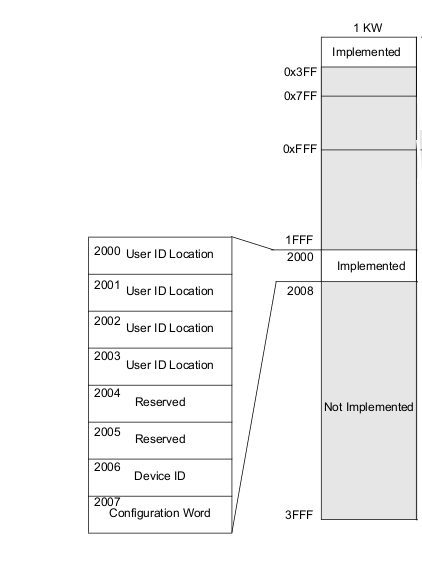
\includegraphics[width=0.4\textwidth]{2017-05-08_at_02:27:50_screenshot.png}
    \caption{Карта памяти микроконтроллера PIC 16f628a. Белым выделены области для пользовательского кода.}
\end{figure}

\textbf{В пространство конфигурационной памяти}
(адреса 0х2000 - 0х2007) можно попасть через передачу в PIC специальной команды 
"Загрузить даннные для конфигурационной памяти". Только адреса 0x2000-0x200F 
конфигурационного пространства памяти физически реализованы. Однако, только 
ячейки 0x2000 вплоть до 0x2007 доступны для программирования. Остальные ячейки
зарезервированны. Переход по адресу за пределами 0x200F будет физически осуществлять
доступ к пользовательской памяти.

\textbf{Пространство ПЗУ памяти}
простирается от 0x00 до 0xFF и находится отдельно от пространства программной памяти
и пространства оперативной памяти. Для ПЗУ реализуются только нижние 128 байт
для устройств PIC16F627A/628A, в то время как для PIC16F648A
реализуются все 256 байт. Программирование ПЗУ памяти данных использует тот же программный счетчик
что и для программирования конфигурационной и програмной памяти, однако только нижние биты
декодируется и используются. Поэтому перед программированием ПЗУ необходимо чтобы 
программный счетчик указывал на 0х0000 или 0х2000.

\textbf{Создание структуры} для представления памяти микроконтроллера. 
Ключевым элементом в представлении памяти микроконтроллера является массив 
типа uint16\_t размером с память PIC. В массиве хранится пользовательская программа 
непосредственно перед её побитовой передачей на микроконтроллер. Из 16 битов отведенных под тип uint16\_t для 
хранения данных и команд используются только нижние 8 и 14 байт соответственно.


Для того чтобы ускорить процесс прошивки микроконтроллера вводятся переменные program\_memory\_used\_cells, и program\_memory\_max\_used\_address. Они обозначают общее колличество задействованных программой ячеек памяти, и самый высокий адрес в програмной памяти. Таким образом можно заметить условия при которых можно досрочно закончить программирование програмной памяти PIC и перейти к следующей стадии программирования.

Ниже приведена структура для представления памяти микроконтроллера.

\begin{small}
\begin{verbatim}
struct picmemory {
    uint16_t  program_memory_used_cells;
    uint16_t  program_memory_max_used_address;

    uint8_t   has_configuration_data;
    uint8_t   has_eeprom_data;

    uint16_t *data;     /* 14-bit and 8-bit data */
    uint8_t  *filled;   /* 1 if this cell is used */
};
\end{verbatim}
\end{small}

\textbf{Внутренний програмный}
счетчик может увеличиваться от 0х0000 до 
конца реализованной програмной памяти 0х03FF (или 0x07FF, или 0x0FFF в зависимости от модели PIC)
после чего он вновь обернется на адресс 0х0000.
Для включения высоких бит програмного счетчика и перехода
к программированию конфигурационной памяти, необходимо послать спецальную команду.
Послее нее програмный счетчик будет оперировать в пространстве от 0х2000 до 0х3FFF
(по достижении 0х3FFF он будет вновь оборачиваться на 0х2000). Единственным 
способом сбросить верхние биты програмного счетчика вновь на 0х0000 это покинуть и
повторно войти в режим программирования.

\textbf{Ячейки для ID}
пользователя отображаются на адреса [0x2000 : 0x2003] и являются 
частью конфигурционной памяти. Пользователь может хранить 
идентификационные данные (идентификатор пользователя) в
четырех локациях для идентификатора пользователя. Этот идентификатор всегда можно считать
корректно, даже если будет включена защита кода.

\textbf{Питание}
в режиме программирования. Для PIC16F627A/628A/648A требуется один источник питания с VDD 
(2.0V до 5.5V) и VPP от 12В до 14В, или же VPP от 4.5В до 5.5В, 
при использовании низковольтного программирования. 
Оба источника должны иметь разрешение как минимум в 0,25В. В данной работе 
используется режим низковольтного программирования.

\textbf{Команды программирования} 
в режиме программирования, обмен информацией с PIC определяеться набором команд и 
их операндами которые передаются в микроконтроллер и/или обратно через серийные кабели. 
Общая форма для всех последовательностей команд
состоит из 6-битовой команды и условно 16-битного
слова данных. И команды и слова данных передаются начиная с наименее значимого бита (LSB first).
Для других серий и линеек типа PIC набор команд может отличаться.

\begin{figure}[h!]
    \centering
    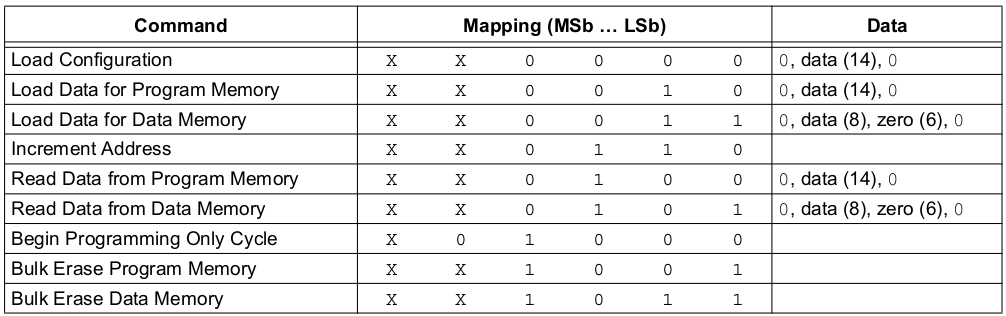
\includegraphics[width=0.8\textwidth]{2017-05-08_at_03:31:35_screenshot.png}
    \caption{Последовательности 6-разрядных команд для PIC16F627A/628A/648A}
\end{figure}

\textbf{I/O Выходы} используемые для программирования. Положительный входной сигнал на ножке RB4 называемой PGM вводит микроконтроллер в режим низковольтного программирования (если данная опция была включена в конфигурационном слове микроконтроллера). Ножка RB7 называемая DATA, настраивается как вход и используется для по-битовой передачи данных программых в микроконтроллер. Ножка RB6 называемая CLOCK, также настраивается на прием входного сигнала и используется для синхронизации состояния напряжения на ножке RB7. Во время падения напряжения на ножке RB6, микроконтроллер считает следующий бит с ножки RB7. Ножка MCLR/Vpp изпользуется для выбора режима программирования. В PIC16F627A/628A/648A, высокое напряжение для работы с ячейками памяти генерируется автоматически. Для активации
режима программирования, необходимо применить высокое напряжение ко входу MCLR. Поскольку MCLR используется на уровне источника, это означает, что MCLR не тянет какиой-либо значительный ток. Ножка VDD предоставляет 5В необходимые для стабильной работы микроконтроллера в штатном режиме. Ножка VSS определяет напряжение на уровне земли.

\begin{figure}[h!]
    \centering
    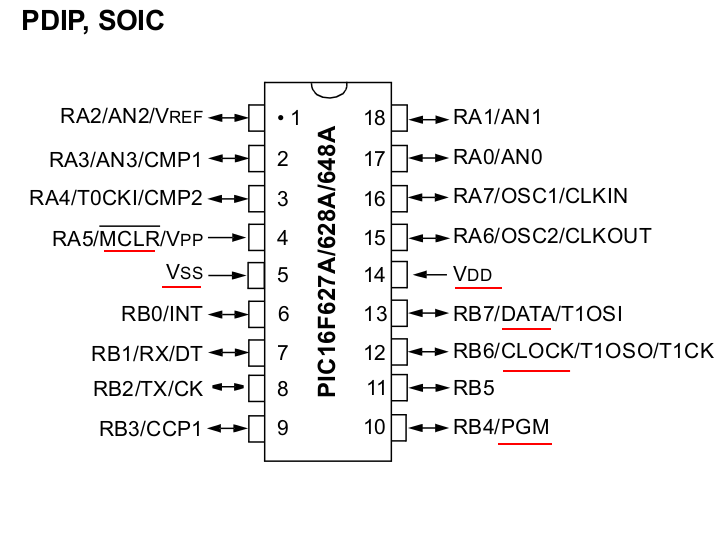
\includegraphics[width=0.8\textwidth]{2017-05-07_at_22:31:52_screenshot.png}
    \caption{I/O выходы необходимые для программирования в серийном режиме}
\end{figure}


\textbf{Абстрагирование программатора} от конкретной модели микроконтроллера семейства PIC 
делается с помощю определения дополнительной структуры в которой для каждой конкретной модели 
хранится информация о карте памяти, о командах программирования, о задержках необходимых между 
сигнальными последовательностями.

\begin{small}
\begin{verbatim}
struct picmicro {
    uint16_t device_id;
    char     name[16];
    size_t   program_memory_size;
    size_t   data_memory_size;

    int program_cycle_time;     /* in microseconds */   // T_PROG
    int eeprom_program_cycle_time;  // T_DPROG
    int bulk_erase_cycle_time;      // T_ERA

    uint8_t load_configuration_cmd;
    uint8_t load_data_for_program_memory_cmd;
    uint8_t load_data_for_data_memory_cmd;
    uint8_t read_data_from_program_memory_cmd;
    uint8_t read_data_from_data_memory_cmd;
    uint8_t increment_address_cmd;
    uint8_t begin_erase_programming_cycle_cmd;
    uint8_t begin_programming_only_cycle_cmd;
    uint8_t bulk_erase_program_memory_cmd;
    uint8_t bulk_erase_data_memory_cmd;
};
\end{verbatim}
\end{small}

Для микроконтроллеров PIC16F627A/628A/648A используется нижеследующее определение экземпляра данной структуры.
\begin{small}
\begin{verbatim}
const struct picmicro pic16f628a = {
    /* General */
    .device_id =                              0x1060,
    .name =                                   "pic16f628a",
    .program_memory_size =                    0x800,
    .data_memory_size =                       128,
    
    /* Time intervals in microseconds */
    .program_cycle_time =                     4000,
    .eeprom_program_cycle_time =              6000,
    .bulk_erase_cycle_time =                  6000,
    
    /* Commands */
    .load_configuration_cmd =                 0x00,
    .load_data_for_program_memory_cmd =       0x02,
    .load_data_for_data_memory_cmd =          0x03,
    .read_data_from_program_memory_cmd =      0x04,
    .read_data_from_data_memory_cmd =         0x05,
    .increment_address_cmd =                  0x06,
    .begin_erase_programming_cycle_cmd =      0xFF,
    .begin_programming_only_cycle_cmd =       0x08,
    .bulk_erase_program_memory_cmd =          0x09,
    .bulk_erase_data_memory_cmd =             0x0B
};
\end{verbatim}
\end{small}


%=============================================================
\subsubsection{Описание алгоритма}

\textbf{Чтение файла} с программой пользователя, это первый шаг программатора. Следующим шагом 
являеться проверка входного файла на корректность. Для этого используются особенности формата INTEL HEX8M.
В частности приведенные в конце строки проверочные суммы и адреса для данных.

\begin{figure}[h!]
    \centering
    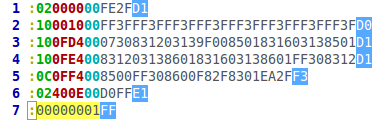
\includegraphics[width=0.6\textwidth]{negated_intel_hex_colored_file_example.png}
    \caption{Пример входного файла к программатору}
\end{figure}


По мере чтения входного файла в соответствующий адрес в массиве структуры "picmemory" вставляются значения из входного файла. 
Поскольку на тонком клиенте Orange Pi Lite установлен little-endian процессор 
компании Allwinner модели H3, а в формате INTEL HEX8M данные записываются в порядке 
MSB, то при вставке в массив необходимо поменять местами верхний и нижний байты.

В цикле происходит прочтение входного файла и создание структуры для представления памяти микроконтроллера, а также подсчет проверочных значений.
\begin{small}
\begin{verbatim}
for (i = 0; i < byte_count / 2; i++) {
        nread = sscanf(&line[9+4*i], "%4hx", &data);
	        uint16_t pic_data = swap_uint16(data);
        if (nread != 1) {
                fprintf(stderr, "Error: cannot read data.\n");
                free_picmemory(&pm);
                return NULL;
        }
        if (debug)
                fprintf(stderr, "  data        = 0x%04X (file) = 0x%04X (micro)\n", data, pic_data);
        checksum_calculated += (data >> 8) & 0xFF;
        checksum_calculated += data & 0xFF;

        if (address + i < 0x2000) {
                pm->program_memory_used_cells       += 1;
                pm->program_memory_max_used_address  = address + i;
        } else if (0x2000 <= address + i && address + i < 0x2008)
                pm->has_configuration_data = 1;
        else if (address + i >= 0x2100)
                pm->has_eeprom_data = 1;

        pm->data[address + i]   = pic_data;
        pm->filled[address + i] = 1;
}
\end{verbatim}
\end{small}

Программатор работает через посылание 
последовательности команд и данных, введенных в серийном режиме
в котором бит на линии данных загоняется в микроконтроллер на падающем
фронте напряжения на линии часов. Команда + данные, вводятся последовательно, 
через линию часы и линию данных, которые с аппаратной точки зрения являются входными линиями 
изпользующими триггеры Шмитта для различения напряжения 0 или 1. 

\begin{figure}[h!]
    \centering
    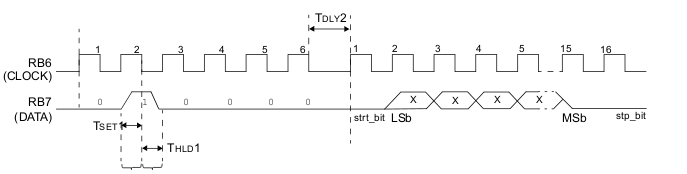
\includegraphics[width=0.8\textwidth]{2017-05-09_at_09:32:56_screenshot.png}
    \caption{Временные интервалы для побитовой передачи команды "Загрузка данных в програмную память"}
\end{figure}

\newpage

\textbf{Минимальные время} установки и удержания приписываются каждому сигнал на ножке данных 
(описанные в таблице ниже, вместе с ограничением по напряжению) по
отношению к падающему фронту напражения на линии часов. Командам на чтение и запись, которые
требуют передачи данных связанных с ними,
требуется минимальная задержка между передачей команды и передачей данных.

\begin{figure}[h!]
    \centering
    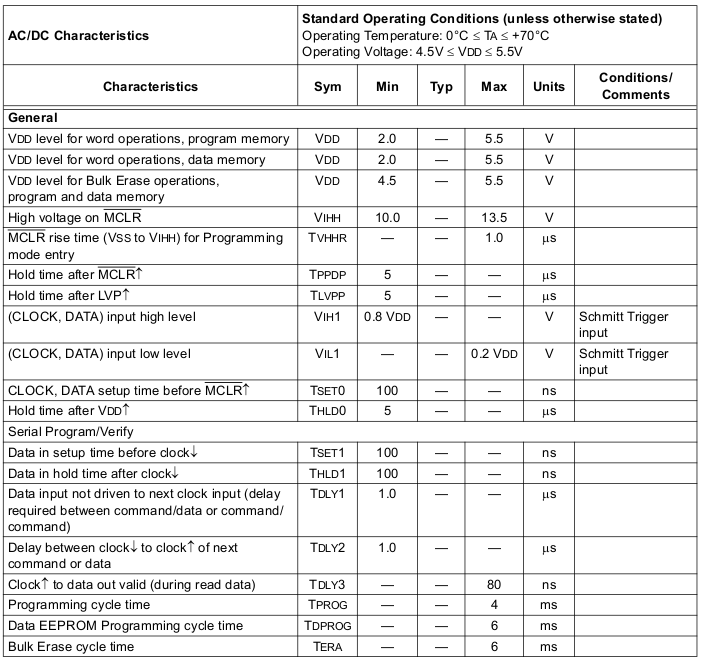
\includegraphics[width=0.8\textwidth]{2017-05-08_at_03:39:19_screenshot.png}
    \caption{Спецификация AC/DC для поднятия/опускания и удержания линий данных и часов}
\end{figure}

\newpage

\textbf{Aлгоритм} записи данных в память программы приведен в нижеследующем графе.

\begin{figure}[h!]
    \centering
    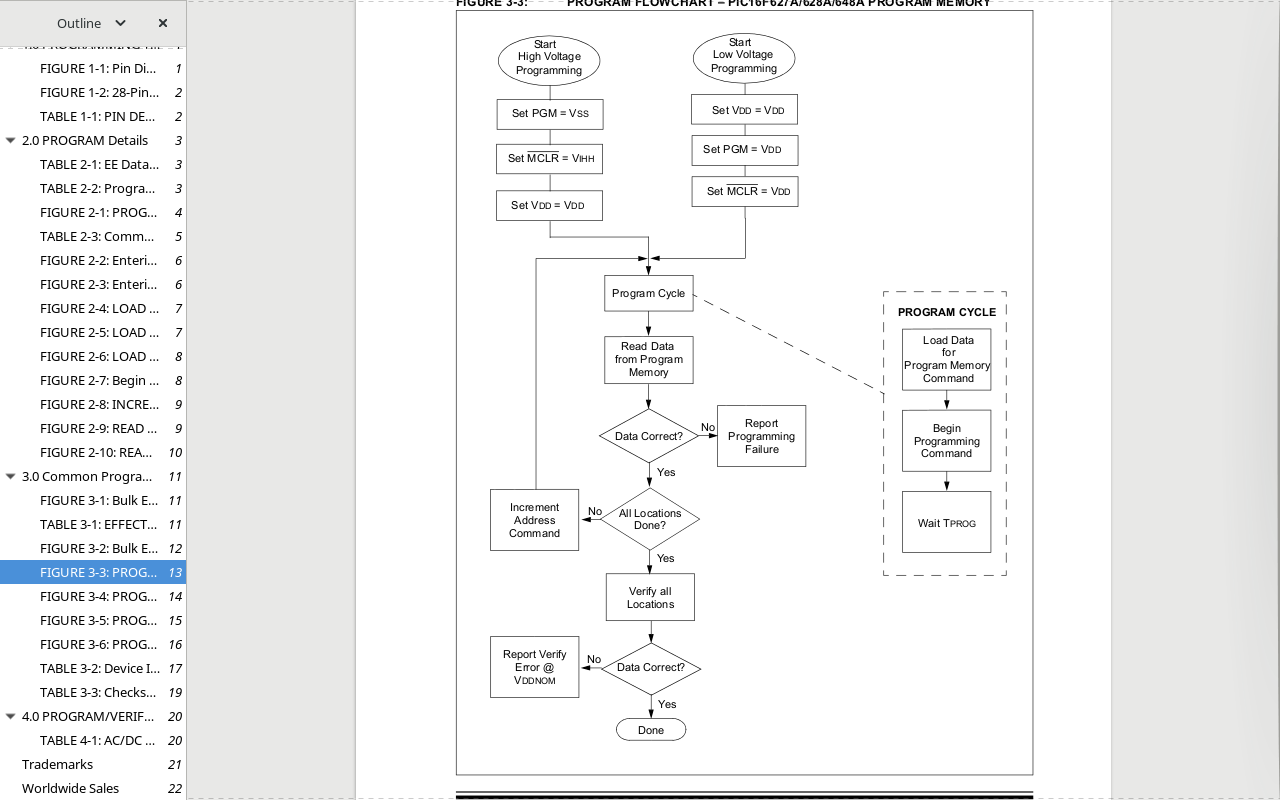
\includegraphics[width=0.8\textwidth]{2017-05-08_at_03:42:09_screenshot.png}
    \caption{Граф алгоритма записи данных в програмную память микроконтроллера}
\end{figure}


\textbf{После создания} карты памяти которая должна быть загруженна в микроконтроллер, следующим 
шагом является непосредственная передача этих данных в PIC. Для этого необходимо получить доступ 
к GPIO выходам тонкого клиента Orange Pi Lite. Со стороны Orange Pi Lite надо было посмотреть на 
поставляемую с ним схемотехнику платы чтобы определить какие выходы PGIO наиболее подходят для работы программатора.
Сигналы передаваемые на ножки микроконтроллера имеют строгие временные рамки, и для того что бы в них вписаться необходимо 
использовать механизм "memory mapped file" для включения и отключения сигналов нв выходах GPIO на уровне процессора.

\begin{figure}[h!]
    \centering
    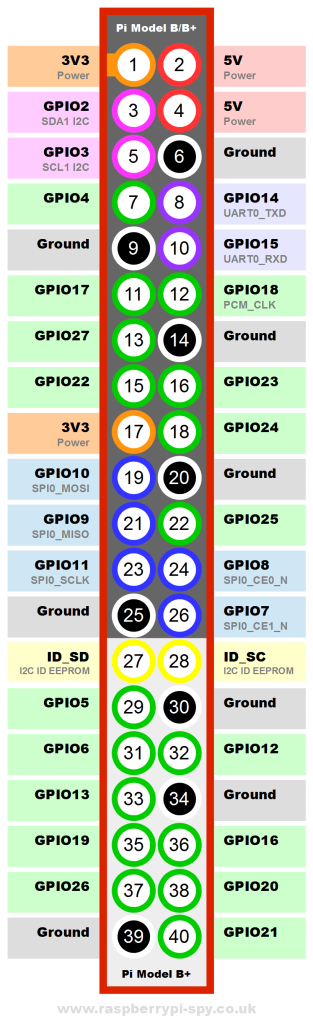
\includegraphics[width=0.25\textwidth]{Raspberry-Pi-B-Plus.png}
    \caption{Разъем GPIO выходов модели Rasberry Pi B+ которая таже используется и на Orange Pi Lite}
\end{figure}

Посмотрев на схемотехнику для выходов GPIO, решено было выбрать 5 последовательных 
выходов 29, 31, 33, 35, 37 которые подсоедены к процессору Н3 соответственно на ножках 7, 8, 9, 10, 20 порта А. 

\begin{figure}[h!]
    \centering
    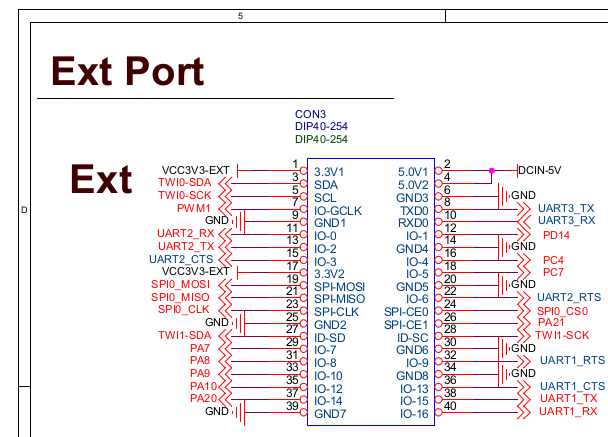
\includegraphics[width=0.8\textwidth]{2017-05-09_at_17:08:33_screenshot.png}
    \caption{Схемотехника для выходов GPIO Orange Pi Lite с процессором H3}
\end{figure}

Из схемотехники ниже понятно что ножки PA7, PA8, PA9, PA10, PA20 подключаются к порту А процессора и выходят на GPIO.

\begin{figure}[h!]
    \centering
    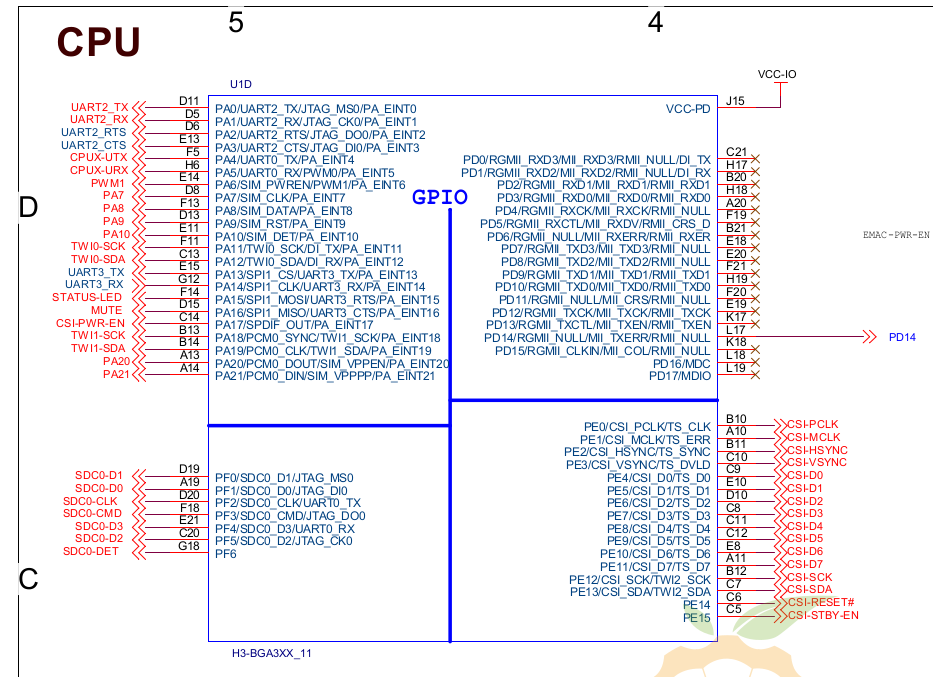
\includegraphics[width=0.8\textwidth]{2017-05-09_at_17:08:43_screenshot.png}
    \caption{Схемотехника для процессора Н3 Orange Pi Lite}
\end{figure}

\newpage

\textbf{Получение доступа} к выходам GPIO, осуществляется через манипуляцию регистрами отвечающими за порт А напрямую. Для этого делаеться маппинг регистров настройки и состояния порта А в адресоное пространство программы. Значения для адресов регистров и их размера берутся из руководства инженера к процессору Н3.
Значения адресов всех регистров влияющих на состояние порта А вписанны в код программы. Далее приведена краткая сводка констант в которые были записаны необходимые адреса.

\begin{small}
\begin{verbatim}
// AllWinner H3 datasheet, page 86, page 316
uint32_t CCU_BASE = 0x01C20000ul;       // Port controller
uint32_t PIO_OFS =  0x00000800ul;       // GPIO offset

// AllWinner H3 datasheet, page 86, block size is 1024 = 1K = 0x400 bytes 
uint32_t PIO_MAP_LEN = 0x2000;          // Port controller end (0x01C20BFF) - Port controller start (0x01C20800)

// AllWinner H3 datasheet, page 316
uint32_t PA_CFG0_OFS = 0x00000000ul;    //  Port A Configure Register 0
uint32_t PA_CFG1_OFS = 0x00000004ul;    //  Port A Configure Register 1
uint32_t PA_CFG2_OFS = 0x00000008ul;    //  Port A Configure Register 2
uint32_t PA_DAT_OFS  = 0x00000010ul;    //  Port A Data Register
\end{verbatim}
\end{small}


Следом были написанны функции для манипулирования этими регистрами. Ниже приведены фрагменты функций которые ипользуются чтобы выставить состояние ножки GPIO на выход (output) и чтобы менять напряжение на дфнной ножке с 0В до 3.3В. Для регистров бит 0 - это наименее значимый бит.


Ниже приведены фрагменты функций которые ипользуются чтобы выставить состояние ножки GPIO на выход (output) и чтобы менять напряжение на дaнной ножке с 0В до 3.3В. Для регистров бит 0 - это наименее значимый бит.

\begin{small}
\begin{verbatim}
// получение указателя на адрес по которому хранится регистр 
volatile uint32_t* get_data_reg(int pin)
{
    volatile uint32_t* data_reg = (volatile uint32_t * )(gpio + PA_DAT_OFS);
    return data_reg;
}

// создает новое измененное значение для записи в регистр
uint32_t modify_data(uint32_t data, int pin, int value)
{
    uint32_t new_data;
    if (value) {
        new_data = data | (1U << pin);
    }
    else {
        new_data = data & ~(1U << pin);
    }
    return new_data;
}

// выставляет на ножке номер "pin" значение напряжения 0 или 1.
void gpio_wr(int pin, int value) {
    volatile uint32_t* data_reg = get_data_reg(pin);
    uint32_t data = *data_reg;
    uint32_t new_data = modify_data(data, pin, value);
    *(data_reg) = new_data;
}

// модифицирует копию текущих настроек чтобы ножка номер "pin" оказалась настроена как ВЫХОД
// возвращает новое значение которое должно быть записано в регистр
uint32_t modify_cfg_output(uint32_t cfg, int pin)
{
    /* Write value 001 to position of pin, each pin is z001 ('z' is dont care) */
    uint32_t new_cfg = cfg & ~(6U << 4 * (pin % 8));
    uint32_t new_new_cfg = new_cfg | (1U << 4 * (pin % 8));
    return new_new_cfg;
}


// модифицирует регистр настроек порта А чтобы ножка номер "pin" оказалась настроена как ВЫХОД
// Pin is one of PA7, PA8, PA9, PA10, PA20
void gpio_output(int pin)
{
    volatile uint32_t* cfg_reg = get_cfg_reg(pin);
    uint32_t cfg = *cfg_reg;
    uint32_t new_cfg = modify_cfg_output(cfg, pin);
    *(cfg_reg) = new_cfg;
}


// модифицирует копию текущих настроек чтобы ножка номер "pin" оказалась настроена как ВХОД
// возвращает новое значение которое должно быть записано в регистр
uint32_t modify_cfg_input(uint32_t cfg, int pin)
{
    /* Write value 000 to position of pin, each pin is z000 ('z' is dont care) */
    uint32_t new_cfg = cfg & ~(7U << 4 * (pin % 8));
    return new_cfg;
}


// модифицирует регистр настроек порта А чтобы ножка номер "pin" оказалась настроена как ВХОД
// Pin is one of PA7, PA8, PA9, PA10, PA20
void gpio_input(int pin)
{
    volatile uint32_t* cfg_reg = get_cfg_reg(pin);
    uint32_t cfg = *cfg_reg;
    uint32_t new_cfg = modify_cfg_input(cfg, pin);
    *(cfg_reg) = new_cfg;
}
\end{verbatim}
\end{small}


\textbf{Последним шагом} произходящим на уровне программы необходимо пройтись по созданной карте памяти микроконтроллера и посылая в PIC команд и их операнды через GPIO передать в 
микророконтроллер необходимую информацию.


\begin{small}
\begin{verbatim}

// Bulk erase the chip, and then write contents of the .hex file to the PIC
void pic_write(const struct picmicro *pic, char *infile, int debug)
{
    uint16_t addr;
    struct picmemory *pm;

    pm = read_inhx16(infile, debug);

    /* Turn pic on. Give supply power. */
    pic_enter_lvp();

    /* Bulk erase the chip first */
    pic_bulk_erase(pic, debug);

    /* Write Program Memory */
    for (addr = 0; addr <= pm->program_memory_max_used_address; addr++) {
        if (pm->filled[addr]) {
            pic_send_cmd(pic->load_data_for_program_memory_cmd);
            pic_load_data(pm->data[addr]);
            // trigger
            pic_send_cmd(pic->begin_programming_only_cycle_cmd);
            usleep(pic->program_cycle_time);
        }
        pic_send_cmd(pic->increment_address_cmd);
    }

    /* Write Configuration Memory */
    if (pm->has_configuration_data) {
        pic_send_cmd(pic->load_configuration_cmd);
        pic_load_data(pm->data[0x2000]);
        for (addr = 0x2000; addr < 0x2008; addr++) {
            if ((addr <= 0x2003 || addr == 0x2007) && pm->filled[addr]) {
                pic_send_cmd(pic->load_data_for_program_memory_cmd);
                pic_load_data(pm->data[addr]);
                // trigger
                pic_send_cmd(pic->begin_programming_only_cycle_cmd);
                usleep(pic->program_cycle_time);
            }
            pic_send_cmd(pic->increment_address_cmd);
        }
    }
    
    pic_exit_lvp();
    free_picmemory(&pm);
}
\end{verbatim}
\end{small}



\subsection{Mетод организации входных и выходных данных}

\subsubsection{Описание метода входных и выходных данных}
Входными данными для работы программатора являются скомпилированный файл программы, микроконтроллер подключенный к плате, а также (для обеспечения взаимодействия с пользователем) клавиатура и/или мышь. Входной файл данных может быть созданн в любой среде разработки и любым компилятором поддершивающим формат INTEL HEX8M. Примером такой среды разработки является MPLAB X (https://www.microchip.com/, разработчик: коммерческая организация Microchip Ltd.).

\begin{my_enumerate}
\item Из-за огромного количества серий микроконтроллеров поддерживать их все не представляется возможным. Поэтому программатор работает только с микроконтроллерами PIC серии 16F, конкретно с линейками 627A / 628A / 648A.
\item Входной файл программы должен соответствовать формату INTEL HEX8M. По сравнению с двумя другими часто встречающимися форматами INTEL HEX8S, INTEL HEХ32, данный формат наиболее оптимально подходит под серию 16F. В силу того что память 14-битных микроконтроллеров не превышает 64 килобайт (здесь подходит формат HEX32) и програмное слово не нуждаеться в разбиении на высокий и низкий байт как в 16-битных микроконтроллерах (здесь подходит формат HEX8S).
\item Пользователь имеeт возможность модифицировать следующие входные данные в процессе работы программы в усливиях графического интерфейса и перед запуском программы в командной строке:
\begin{my_enumerate}
\item Указать что требуется запись EEPROM памети без модификации програмной памяти микроконтроллера.
\item Указать что требуется проверить входной файл на ошибки.
\item Указать что требуется записать входной файл в програмную память и в EEPROM память микроконтроллера.
\item Поменять уровень колличества сообщений выводимих программой пользователю.
\item Отменить процесс программирования.
\end{my_enumerate}
\end{my_enumerate}

\medskip
Выходными данными для программатора является запрограммированный микроконтроллер, данные на экране и индикатор программирования на плате программатора.


\subsection{Выбор состава технических средств}

\subsubsection{Состав технических и програмных средств}
Для оптимальной работы приложения необходимы следующие системные требования:
\begin{my_enumerate}

\item Тонкий клиент Orange Pi Lite, оснащенный:
    \begin{my_enumerate}
    \item Обязательно процессор Allwinner H3 с тактовой частотой 1 гигагерц (ГГц) или выше;
    \item 0.5 ГБ оперативной памяти (ОЗУ);
    \item 0.5 ГБ свободного места на жестком диске;
    \item Периферия: выход GPIO типа Rasberry Pi B+
    \end{my_enumerate}
\item Опционально: Компьютер для удаленного доступа к Orange Pi Lite, оснащенный:
    \begin{my_enumerate}
    \item Обязательно 64-разрядный (x64) процессор с тактовой частотой 1 гигагерц (ГГц) или выше;
    \item 1 ГБ оперативной памяти (ОЗУ);
    \item 1.5 ГБ свободного места на жестком диске;
    \item Wifi модулем (если Orange Pi Lite подключен к сети, то можно воспользоваться и стандартным Ethernet портом) или TTL переходником для подключения к тонкому клиенту Orange Pi Lite.
    \end{my_enumerate}
\item Монитор
\item Мышь
\item Клавиатура
\end{my_enumerate}
